\section{Design Goals}
\subsection{Purpose}
The purpose of this software project is to create a simulation within Unity to recreate real-time traffic scenarios. By focusing on real-time traffic data collection, different pathfinding algorithms, with visualization help of Unity, the project aims to provide users with a platform for comparing simulated traffic behaviors to real-life situations.
\subsection{Objectives}
Our initial goals for the project included:

\begin{enumerate}
	\item Real-Time Traffic Data Collection:
	Collect real-time data from satellite imagery to construct maps for the simulation.
	\item Pathfinding:
	Implementing pathfinding algorithms to simulate realistic vehicle movements and route optimization within the traffic simulation.
	\item Rendering in Unity with 3D Objects:
	Utilizing Unity's to create visual representations of the simulated traffic scenarios.
\end{enumerate}
\textbf{ Were they met? Why/Why not?}

Due to the project's complexity and time constraints, some of our initial goals were not fully met
\begin{enumerate}
	\item Real-Time Creation of Map with Data: While we did integrate real-time data collection mechanisms, such as traffic APIs through TomTom, into the project, the process of dynamically constructing maps within the simulation environment proved more challenging than originally believed. As a result, the maps were often pre-generated and simplified representations rather than real-time creations.
	\item Real-Time Comparison to Traffic: Achieving real-time comparison to real-life traffic was a significant challenge. Despite implementing a pathfinding algorithm and system, accurately recreating the complexities of real-world traffic behaviors within the Unity environment proved to be beyond the project's scope within the given timeframe.
	\item Different Pathfinding Algorithms: While we implemented several pathfinding algorithms, such as Dijkstra's algorithm and A* search, integrating a wide range of algorithms for comparative analysis was not feasible within the project's constraints.
\end{enumerate}
However the project did accomplish in other main areas
\begin{enumerate}
	\item Visualization: Overall, the visualization and creation of the different assets for the project in order to show a visually appealing simulation to the user
	\begin{figure}[htbp]
	    \centering
	    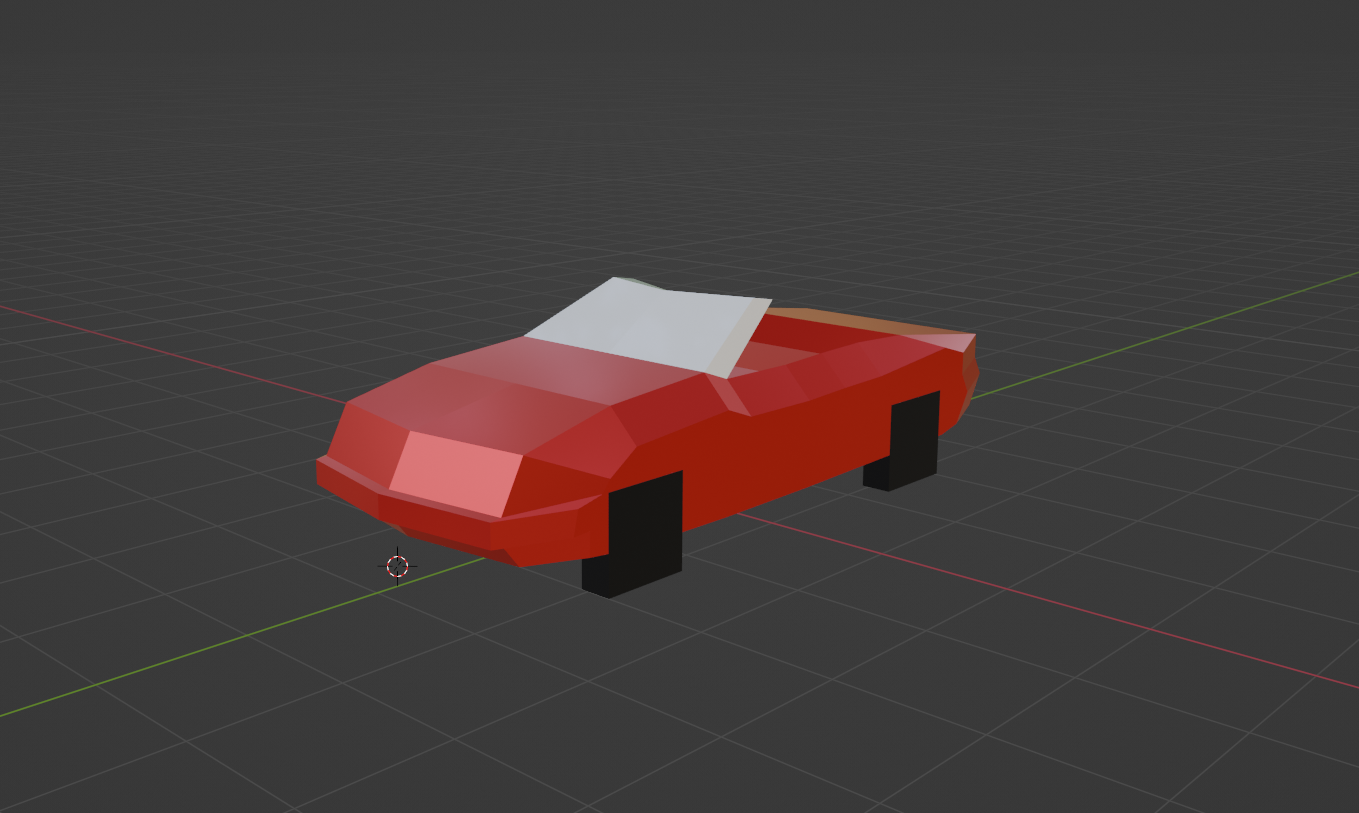
\includegraphics[width=0.5\textwidth]{Images/SportsCar.png}
	    \caption{Sports Car rendered in Blender}
	    \label{fig:SportsCar}
	\end{figure}
	\item Map Creation: With the use of the TomTom API, the project was able to have a few select scenes of nearby areas and which were digitally recreated.
	\begin{figure}[htbp]
	    \centering
	    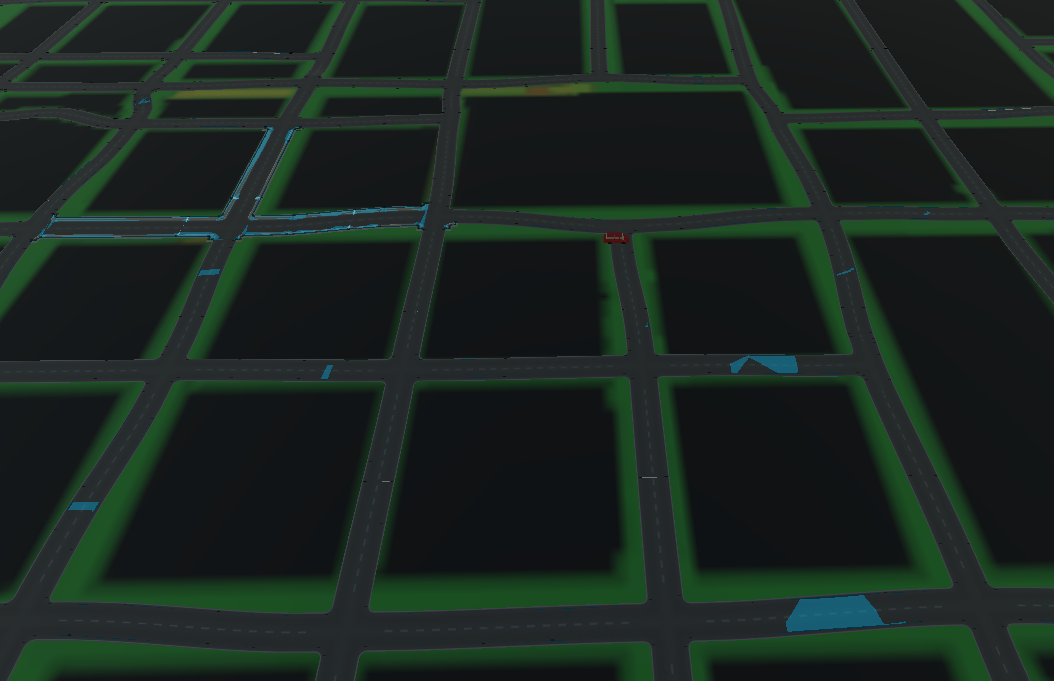
\includegraphics[width=0.5\textwidth]{Images/Map.png}
	    \caption{Map rendered in Unity}
	    \label{fig:Map}
	\end{figure}
	\item Main Pathfinding: The overall scoring of the pathfinding is interesting enough and accurate to normal behavior of traffic. As more vehicles enter the road, congestion will occur and the overall speed to reach the goal is reduced heavily.
\end{enumerate}
\textbf{Comparison to Initial Vision}
Despite falling short, the finished project represents a significant achievement in terms of simulating real-time traffic within a Unity. While compromises were made due to complexity and time constraints, the project still provides valuable insights into traffic simulation and serves as a foundation for future developments to the project.

\begin{flushleft}
Below is a sequential diagram for the design of the code and classes running inside Unity.  The main relationships are between the UI, which are the classes UIManager and PathSet, and the spawns like SpawningCars, SpawnPF, and PathFind that makes the pathfinding algorithm for the main car object. 
\end{flushleft}

\begin{figure}[htb]
    \centering
    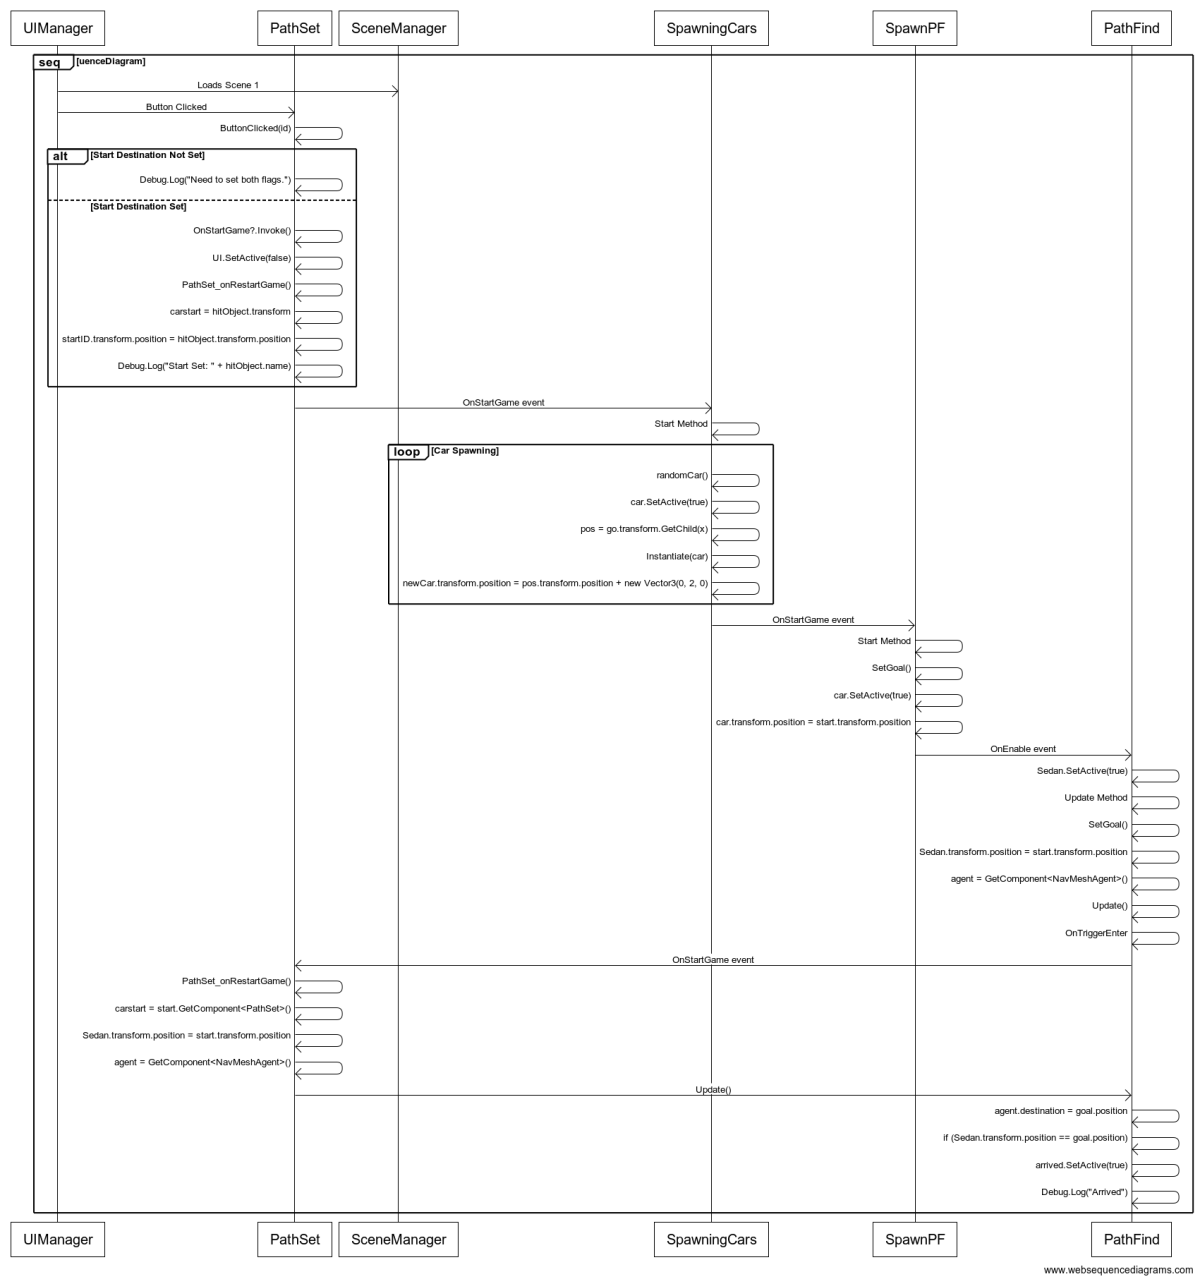
\includegraphics[width=10cm]{Images/Sequential.png}
       \caption{Sequential class diagram.}
           \label{Fig:Game}
\end{figure}